\documentclass[11pt, a4paper]{article}
\PassOptionsToPackage{hidelinks}{hyperref} 
\usepackage[utf8]{inputenc} 
\usepackage{fullpage}
\usepackage{graphicx}
\usepackage{xcolor}
\usepackage{amsmath}
\usepackage{bookmark}
\usepackage{ragged2e}
\usepackage{amsmath}
\usepackage{amsfonts}
\usepackage{array}
\usepackage{float}
\usepackage{tabularx}
\usepackage{listings}
\usepackage{hyperref}
\usepackage[backend=biber]{biblatex}
\renewcommand\UrlFont{\color{blue}\rmfamily}
 
% Title of your project
\title{Prediction with Back-Propagation and Linear Regression }

% Name of deliverable
\newcommand{\deliverableName}{Delivery of Activity 1}

% Author
\author{Javier Novella Ruiz}

% Group number
\newcommand{\groupNumber}{17685106}

% Comment
\newcommand{\comments}{Virtual student}

% Date for title page, default is today and 
\date{\today}

\makeatletter{}

\setlength{\parindent}{0pt}

\begin{document}

\begin{titlepage}
  	\newcommand{\HRule}{\rule{\linewidth}{0.3mm}}
	\center
	%------------------------------------------------
	%	Headings
	%------------------------------------------------
	
	\textsc{\LARGE Universitat Rovira i Virgili}\\[1.5cm]
	
	\textsc{\Large \deliverableName}\\[0.5cm]
	
	\textsc{\large Neural and Evolutionary Computation}\\[0.5cm]
	
	%------------------------------------------------
	%	Title
	%------------------------------------------------
	
	\HRule\\[0.4cm]
	
	{\huge\bfseries \@title}\\[0.4cm]
	
	\HRule\\[1.5cm]
	
	%------------------------------------------------
	%	Author(s)
	%------------------------------------------------

 	{\large\sc\@author}
	
	%------------------------------------------------
	%	Date
	%------------------------------------------------
	
	\vfill\vfill
	%	{\large\@date}
    \vfill\vfill\vfill
	
	%------------------------------------------------
	%	Logo
	%------------------------------------------------
	\vfill
	
\includegraphics[width=0.3\textwidth]{./urvlogo.png}
	\vfill
\end{titlepage}


\tableofcontents

\newpage

\section{Introduction}

The goal of this activity is to practice with different types of supervised models. In particular, the following methods have been used. 
\begin{itemize}
    \item Neural Network with Back-Propagation BP, implemented by the author of this report.
    \item Neural Network with Back-Propagation BP-F, using keras library.
    \item Multiple Linear Regression MLR-F, using the sklearn python library.
\end{itemize}

To achieve this purpose firstly the a dataset has been selected, analyzed and pre-processed. Then the methods commented before have been
applied to the dataset to obtain predictions of values.

\subsection{GitHub repository}

The Jupyter Notebook and the module with the BP devolpemnt together with the dataset files and image results can be consulted in
the following GitHub repository (\href{https://github.com/novella93/NEC_A1}{Link to Javier Novella NEC A1 repository}).

\vspace{1em} From the descriptions and explanations point of view, the Jupyter Notebook file A1.ipynb contains a retailed version of this 
report in the markdowns. But it contains all the Python code used to obtain the results for this report.

\vspace{1em} For the BP implementation the file BP.py is the module which implements the NeuralNet Class, and can be found also in the same
repository.

\section{Dataset}

The dataset used include data for the estimation of obesity levels in individuals from the countries of Mexico, Peru and Colombia, based 
on their eating habits and physical condition. The data contains 17 attributes and 2111 records. The dataset source is UCI Machine Learning 
Repository \href{https://archive.ics.uci.edu/dataset/544/estimation+of+obesity+levels+based+on+eating+habits+and+physical+condition}{(Link to the dataset repository)}.

\vspace{1em} The dataset is composed by the following features:

\begin{itemize}
    \item \textbf{Gender}: gender of the individual.
    \item \textbf{Age}: age of the individual.
    \item \textbf{Height}: height of the individual.
    \item \textbf{Weight}: weight of the individual.
    \item \textbf{family\_history\_with\_overweight}: Has a family member suffered or suffers from overweight?
    \item \textbf{FAVC}: Does the individual eat high caloric food frequently?
    \item \textbf{FCVC}: Does the individual usually eat vegetables in your meals?
    \item \textbf{NCP}: How many main meals does the individual have daily?
    \item \textbf{CAEC}: Does the individual eat any food between meals?
    \item \textbf{SMOKE}: Does the individual smoke?
    \item \textbf{CH20}: How much water does the individual drink daily?
    \item \textbf{SCC}: Does the individual monitor the calories eaten daily?
    \item \textbf{FAF}: How often the individual has physical activity?
    \item \textbf{TUE}: How much time does the individual use technological devices such as cell phone, videogames, television, computer and others?
    \item \textbf{CALC}: How often does the individual drink alcohol?
    \item \textbf{MTRANS}: Which transportation does the individual usually use?
    \item \textbf{NObeyesdad}: Obesity level
\end{itemize}

\subsection{Inputs and output selection}

From the 17 features, 16 of them are considered inputs and 1 is considered output.

\begin{itemize}
    \item \textbf{Inputs:}
    \begin{itemize}
        \item Gender
        \item Age
        \item Height
        \item Weight
        \item family\_history\_with\_overweight
        \item FAVC
        \item FCVC
        \item NCP
        \item CAEC
        \item SMOKE
        \item CH20
        \item SCC
        \item FAF
        \item TUE
        \item CALC
        \item MTRANS
    \end{itemize}
    \item \textbf{Outputs:}
    \begin{itemize}
        \item NObeyesdad
    \end{itemize}
\end{itemize}

\subsection{Output transformation}

The output NObeyesdad allows classification of the data using the values of Insufficient Weight, Normal Weight, Overweight Level I, 
Overweight Level II, Obesity Type I, Obesity Type II and Obesity Type III. As the predicted variable must be a real value \(float or double\) 
this value will be replaced by the corresponding \(BMI\).

\vspace{1em}The Body Mass Index \(BMI\) is a simple calculation using a person's height and weight. The formula is \(BMI = \frac{weight}{height^{2}}\) 
\((\frac{kg}{m^{2}})\). It is used as an indicator of whether an individual is underweight, normal weight, overweight, or obese. The correspondance from the 
previous  categorical values to the new numerical ones are:

\begin{itemize}
    \item \textbf{Insufficient Weight (Underweight)}: BMI less than 18.5
    \item \textbf{Normal Weight}: BMI between 18.5 and 24.9
    \item \textbf{Overweight Level I (Pre-obesity)}: BMI between 25 and 29.9
    \item \textbf{Overweight Level II}: BMI between 30 and 34.9
    \item \textbf{Obesity Type I}: BMI between 35 and 39.9
    \item \textbf{Obesity Type II}: BMI between 40 and 44.9
    \item \textbf{Obesity Type III}: BMI 45 and above
\end{itemize}

To achive this result, the value of the column "NObeyesdad" is replaced by the mentioned formula \(BMI = \frac{weight}{height^{2}}\) using 
the weight and height within the same record processed. This will result in the \(BMI\) calcualted for each individual which is a real numeric value.

\subsection{Dataset checks}

The data will be checked for the following points:

\begin{itemize}
    \item Check for missing values
    \item Check for duplicates
    \item Check data type
    \item Check unique values on each column
\end{itemize}

\subsubsection{Check missing values}

The dataset is fully checked for null values feature by feature. No missing values are found in during this search.

\begin{table}[H]
    \centering
    \begin{tabular}{|c|c|c|}
        \hline
        \textbf{Feature} & \textbf{Number of missing values} \\ \hline
        Gender & 0 \\ \hline
        Age & 0 \\ \hline
        Height & 0 \\ \hline
        Weight & 0 \\ \hline
        family\_history\_with\_overweight & 0 \\ \hline
        FAVC & 0 \\ \hline
        FCVC & 0 \\ \hline
        NCP & 0 \\ \hline
        CAEC & 0 \\ \hline
        SMOKE & 0 \\ \hline
        CH2O & 0 \\ \hline
        SCC & 0 \\ \hline
        FAF & 0 \\ \hline
        TUE & 0 \\ \hline
        CALC & 0 \\ \hline
        MTRANS & 0 \\ \hline
        Nobeyesdad & 0 \\ \hline
    \end{tabular}
    \caption{Number of missing values within the full dataset}
    \label{tab:table_missing_values}
\end{table}

\subsubsection{Check duplicates}

24 records are duplicated. This means that the dataset contains information about 24 individuals that have exactly the same features. 
In this case, this duplicates are kept because it is assumed that they represent legitimate repeated records from different people.

\subsubsection{Check datatypes}

Check data types allows to make a first sight to know which features are numerical and which are categorical. This will help in the further 
pre-processing steps to know which fields must be transformed/normalized. In this case the features are:

\begin{table}[H]
    \centering
    \begin{tabular}{|c|c|c|}
        \hline
        \textbf{Feature} & \textbf{Data type} & \textbf{Type} \\ \hline
        Gender & object & Categorical \\ \hline
        Age & float64 & Numerical \\ \hline
        Height & float64 & Numerical \\ \hline
        Weight & float64 & Numerical \\ \hline
        family\_history\_with\_overweight & object & Categorical \\ \hline
        FAVC & object & Categorical \\ \hline
        FCVC & float64 & Numerical \\ \hline
        NCP & float64 & Numerical \\ \hline
        CAEC & object & Categorical \\ \hline
        SMOKE & object & Categorical \\ \hline
        CH2O & float64 & Numerical \\ \hline
        SCC & object & Categorical \\ \hline
        FAF & float64 & Numerical \\ \hline
        TUE & float64 & Numerical \\ \hline
        CALC & object & Categorical \\ \hline
        MTRANS & object & Categorical \\ \hline
        NObeyesdad & float64 & Numerical \\ \hline
    \end{tabular}
    \caption{Data types of each feature}
    \label{tab:table_data_types}
\end{table}

\subsubsection{Check unique values by feature}

Understanding the range of unique values in categorical variables will help in choosing the right encoding techniques.

\begin{table}[H]
    \centering
    \begin{tabular}{|c|c|c|}
        \hline
        \textbf{Feature} & \textbf{Number of unqiue values} \\ \hline
        Gender & 2 \\ \hline
        Age & 1402 \\ \hline
        Height & 1574 \\ \hline
        Weight & 1525 \\ \hline
        family\_history\_with\_overweight & 2 \\ \hline
        FAVC & 2 \\ \hline
        FCVC & 810 \\ \hline
        NCP & 635 \\ \hline
        CAEC & 4 \\ \hline
        SMOKE & 2 \\ \hline
        CH2O & 1268 \\ \hline
        SCC & 2 \\ \hline
        FAF & 1190 \\ \hline
        TUE & 1129 \\ \hline
        CALC & 4 \\ \hline
        MTRANS & 5 \\ \hline
        Nobeyesdad & 1340 \\ \hline
    \end{tabular}
    \caption{Number of unique values by feature}
    \label{tab:table_unique_values}
\end{table}

\subsection{Statistics}

The dataset consists of 2111 records and 17 features, with each record considered unique despite some duplications. 
Importantly, there are no null values in the dataset, ensuring completeness. The features cover aspects of individuals' health and lifestyle, 
including height, weight, vegetable intake, number of main meals, water consumption, sports activity, use of technological devices, and BMI.

\begin{table}[H]
    \centering
    \begin{tabular}{|c|c|c|c|c|c|c|c|c|c|}
        \hline
              &    Age   & Height   & Weight   & FCVC     & NCP      & CH2O     & FAF      & TUE        & NObeyesdad \\ \hline 
        count &     2111 & 2111     & 2111     & 2111      & 2111    & 2111     & 2111     & 2111       & 2111 \\ \hline
        mean  & 24.310   & 1.700    & 86.590   & 2.420    & 2.690    & 2.010    & 1.010    & 0.660      & 29.700   \\ \hline
        std   & 6.350    & 0.090    & 26.190   & 0.530    & 0.780    & 0.610    & 0.850    & 0.610      & 8.010    \\ \hline
        min   & 14.000   & 1.450    & 39.000   & 1.000    & 1.000    & 1.000    & 0.000    & 0.000      & 13.000   \\ \hline
        25\%  & 19.950   & 1.630    & 65.470   & 2.000    & 2.660    & 1.580    & 0.120    & 0.000      & 24.330   \\ \hline
        50\%  & 22.780   & 1.700    & 83.000   & 2.390    & 3.000    & 2.000    & 1.000    & 0.630      & 28.720   \\ \hline
        75\%  & 26.000   & 1.770    & 107.430  & 3.000    & 3.000    & 2.480    & 1.670    & 1.000      & 36.020   \\ \hline
        max   & 61.000   & 1.980    & 173.000  & 3.000    & 4.000    & 3.000    & 3.000    & 2.000      & 50.810   \\ \hline
    \end{tabular}
    \caption{Statistics from the dataset}
    \label{tab:table_statistics}
\end{table}

\vspace{1em}The dataset shows a range of values for these features. Heights range from 1.45 to 1.98 meters, and weights range from 39.0 to 173.0 kilograms. 
Individuals consume between 1 to 3 pieces of vegetables per day and have 1 to 4 main meals daily. Water intake varies from 1 to 3 liters per day, 
sports activity ranges from 0 to 3 hours per day, and use of technological devices ranges from 0 to 2 hours per day. BMI values span 
from 13.0 to 50.81 kg/m², indicating a wide range of body compositions.

\vspace{1em}In terms of data distribution, the features with the highest variability are age, weight, and obesity level. The averages of these features are 
close to the 50th percentile, suggesting that the data is evenly distributed. This balanced distribution is beneficial for analysis, as it 
indicates that the dataset provides a comprehensive representation of the population's health and lifestyle characteristics.

\subsubsection{Categorical features}

The categorical features and its exposed in the Table \ref{tab:table_categorical_values}.

\begin{table}[H]
    \centering
    \begin{tabular}{|c|c|}
        \hline
        \textbf{Feature} & \textbf{Possible values} \\ \hline
        Gender & ['Female' 'Male'] \\ \hline
        family\_history\_with\_overweight & ['yes' 'no'] \\ \hline
        FAVC & ['no' 'yes'] \\ \hline
        CAEC & ['Sometimes' 'Frequently' 'Always' 'no'] \\ \hline
        SMOKE & ['no' 'yes'] \\ \hline
        SCC & ['no' 'yes'] \\ \hline
        CALC & ['no' 'Sometimes' 'Frequently' 'Always'] \\ \hline
        MTRANS & ['Public\_Transportation' 'Walking' 'Automobile', \\
               & 'Motorbike' 'Bike'] \\ \hline
    \end{tabular}
    \caption{Possible values of the categorical features}
    \label{tab:table_categorical_values}
\end{table}

In the Figure \ref{fig:image_distribution_categorical_features} it shown the distribution of the categorical data. Showing the distribution 
is important when analyzing a dataset for neural network usage because it helps identify imbalances and patterns within the data. This understanding 
can help training on a representative sample, and this can improve its accuracy and generalization. It also shows any potential biases, allowing for 
adjustments to be made to achieve good predictions.

\begin{figure}[H]
    \centering
    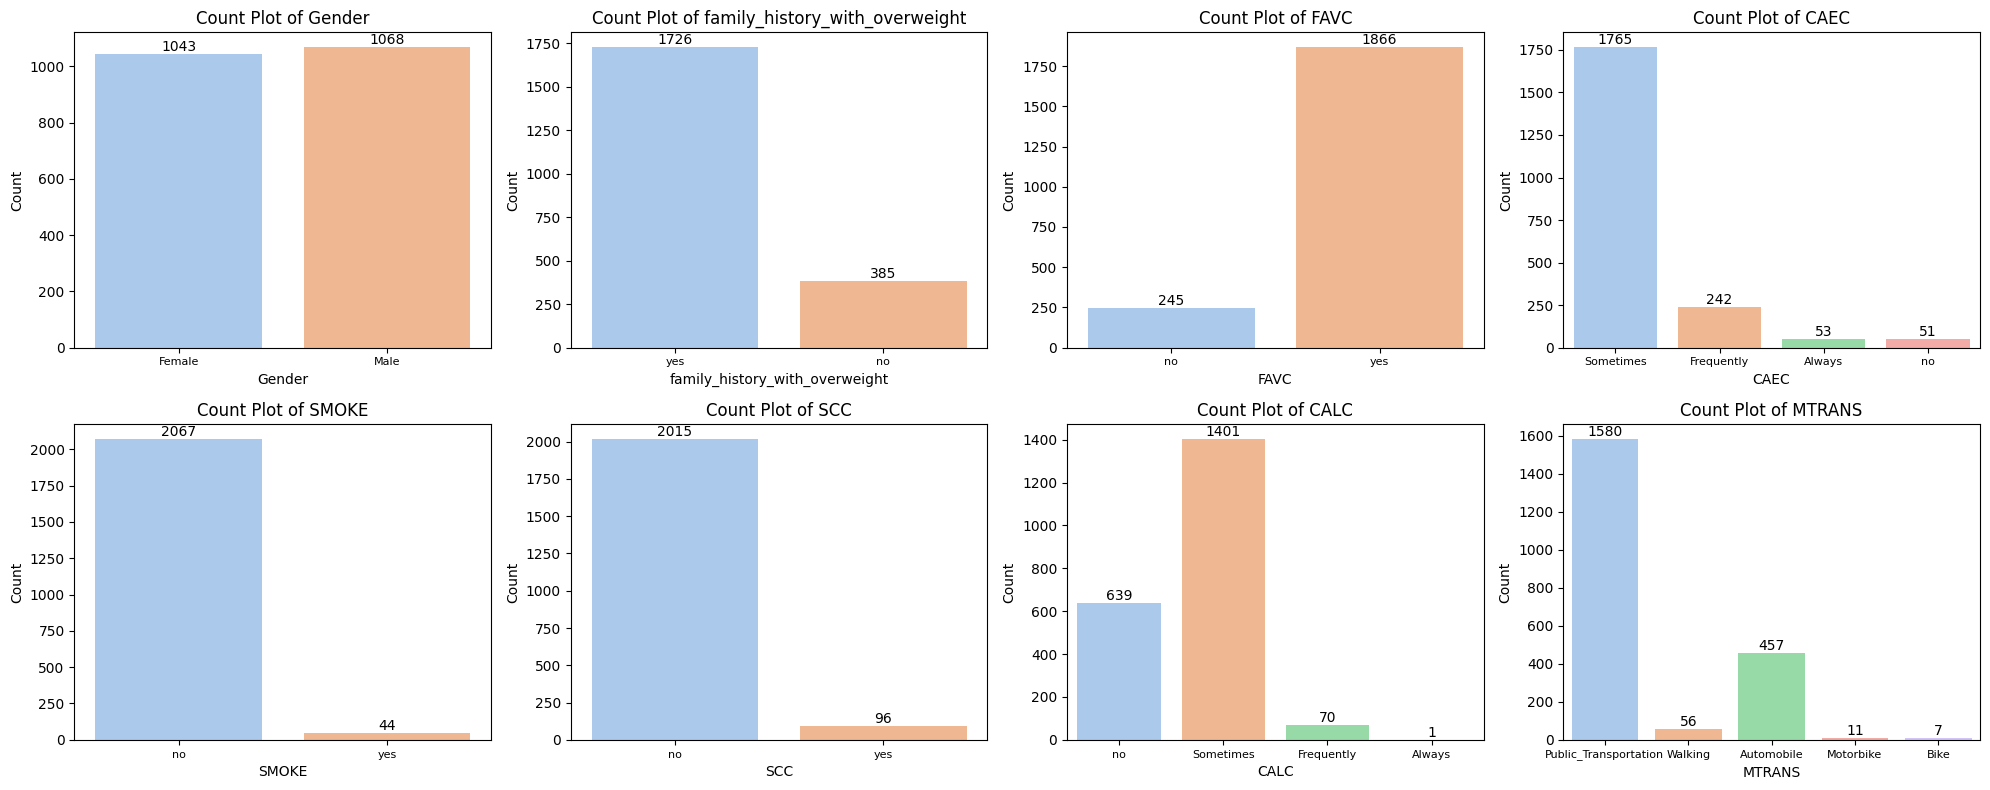
\includegraphics[width=\textwidth]{images/distribution_categorical_features.png}
    \caption{Distribution of the categorical features}
    \label{fig:image_distribution_categorical_features}
  \end{figure}

But the get more insights it is interesting to get the boxplot of the categorical features against the output feature that is the obesity level.
This is shown in the Figure \ref{fig:image_categorical_features_vs_obesity_level}. This view provide a clear summary of the distribution, 
central tendency, and variability of obesity levels within each category. This helps identify patterns, outliers, and differences between groups, 
making it easier to understand how different categorical factors influence obesity.

\begin{figure}[H]
    \centering
    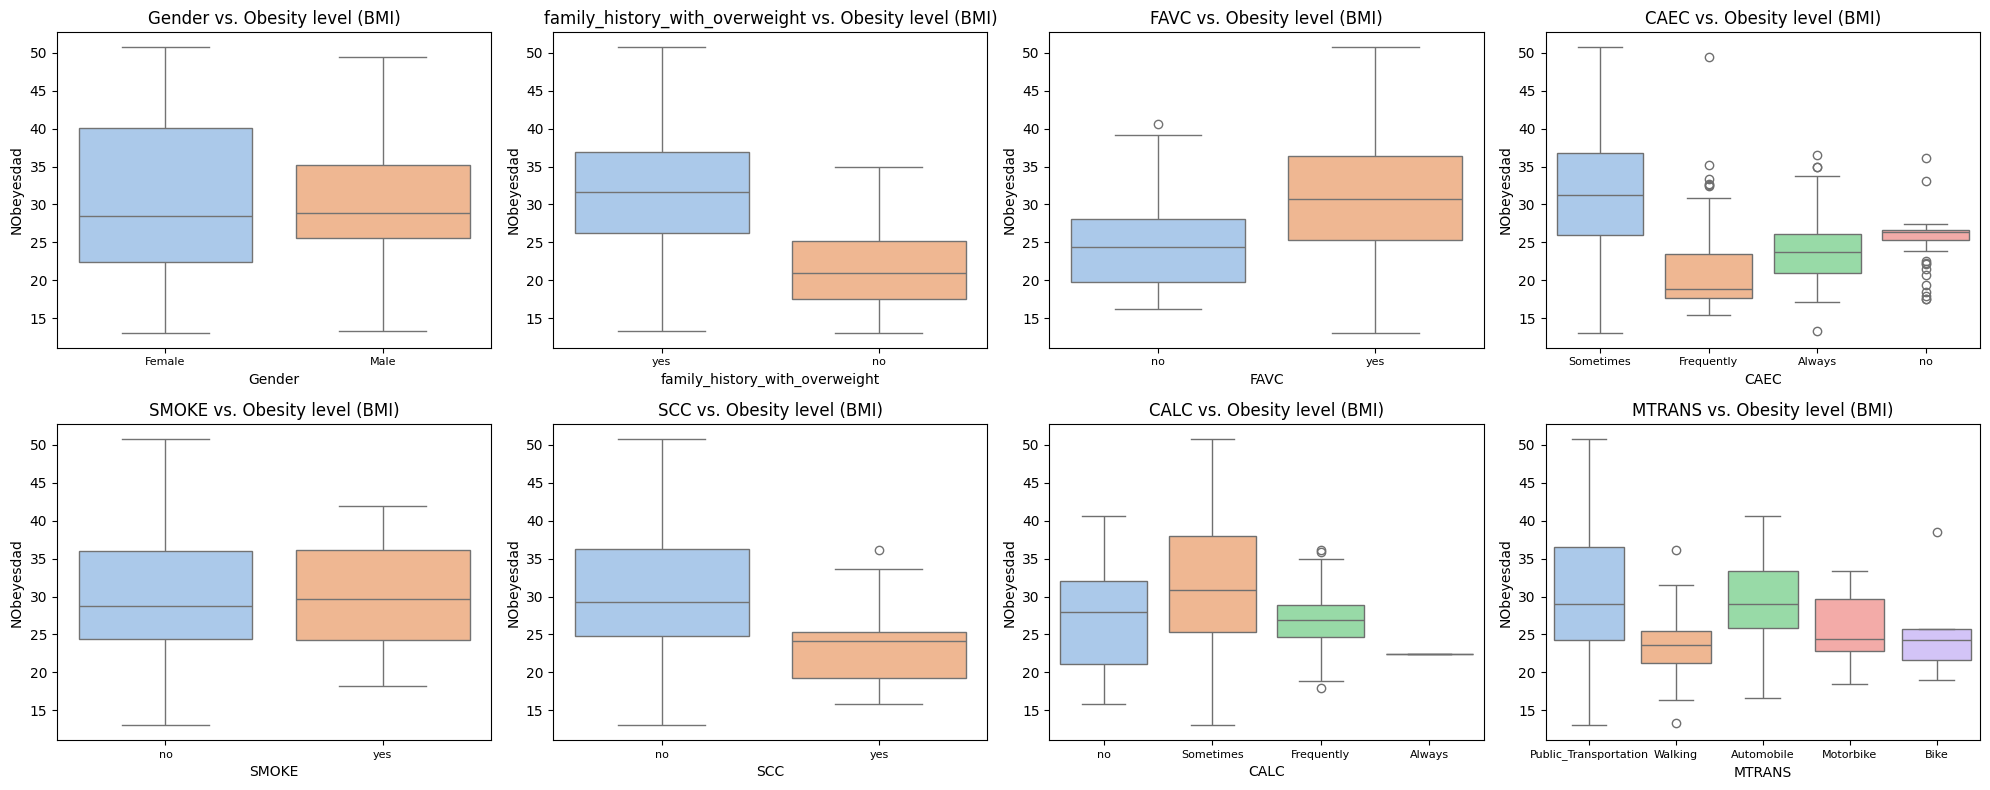
\includegraphics[width=\textwidth]{images/categorical_features_vs_obesity_level.png}
    \caption{Categorical features vs obesity level}
    \label{fig:image_categorical_features_vs_obesity_level}
\end{figure}

From this data, can be exposed that males tend to have higher levels of obesity compared to females. High caloric diets are associated with increased 
obesity levels, while controlling calorie intake helps in maintaining lower obesity levels. Interestingly, smoking does not seem to impact obesity levels 
significantly.

\vspace{1em}Additionally, individuals who use active transportation methods like walking or biking tend to have lower obesity levels. These findings 
highlight the importance of diet and physical activity in managing obesity.

\subsubsection{Numerical features}

In the Figure \ref{fig:image_distribution_numerical_features} it shown the distribution of the numerical data. Showing the distribution of numerical 
features using histograms is important because it helps visualize the data's shape, central tendency, and spread.

\begin{figure}[H]
    \centering
    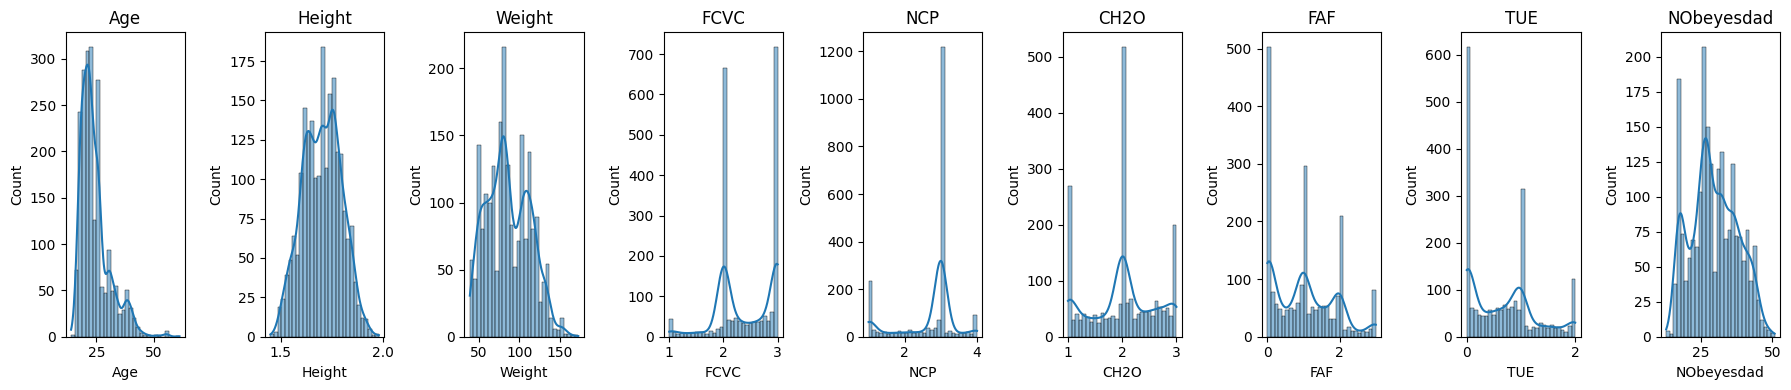
\includegraphics[width=\textwidth]{images/distribution_numerical_features.png}
    \caption{Distribution of the numerical features}
    \label{fig:image_distribution_numerical_features}
\end{figure}

It is interesting to focus on the output variable, to get more insights from the dataset, this is shown in the Figure \ref{fig:image_distribution_obesity_level}.
Focusing on the distribution of the obesity level, is crucial because it helps understand the range and variability of the variable. 

\begin{figure}[H]
    \centering
    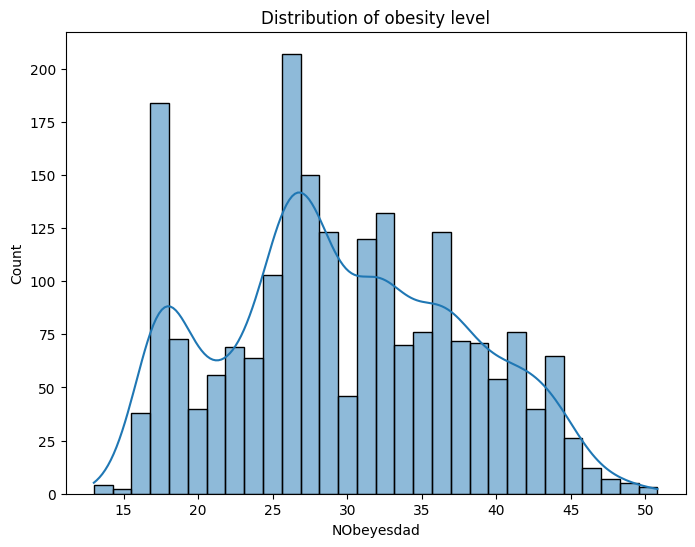
\includegraphics[width=300pt]{images/distribution_obesity_level.png}
    \caption{Distribution of the obesity level}
    \label{fig:image_distribution_obesity_level}
\end{figure}

The relation between this numerical data and its affectance to the output variable can be seen in the correlation matrix shown in the 
Figure \ref{fig:image_correlation_matrix_between_features}. A heatmap of the correlation matrix is used because it visually represents 
the strength and direction of relationships between the numerical features. This helps identify which features are strongly correlated 
with each other and also with the obesity level.

\begin{figure}[H]
    \centering
    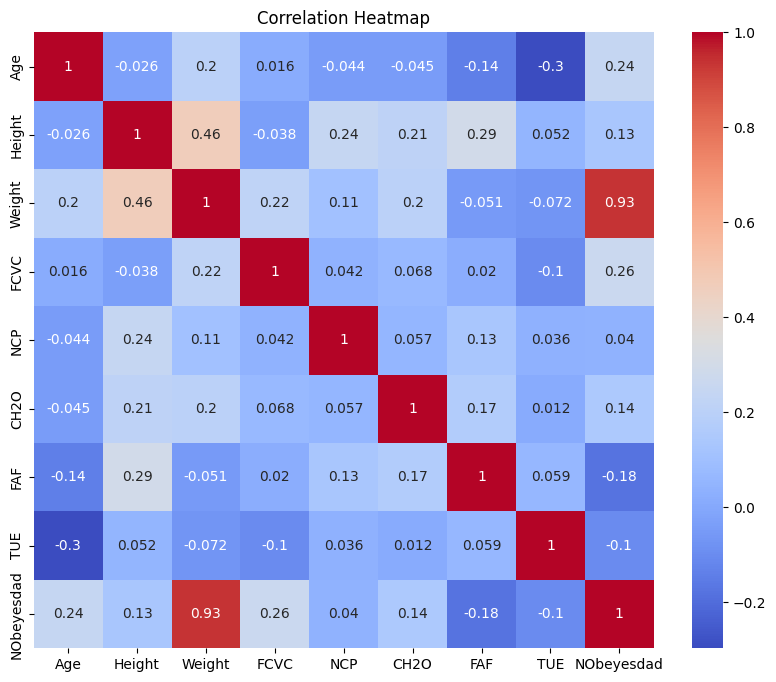
\includegraphics[width=300pt]{images/correlation_matrix_between_features.png}
    \caption{Coorrelation matrix between numerical features}
    \label{fig:image_correlation_matrix_between_features}
\end{figure}

From this data is deduced taht the individuals in the dataset have a BMI ranging from 13.0 to 50.81 kg/m². The average obesity level is 29.7, 
which corresponds to Overweight Level I, close to the threshold for Overweight Level II. It is important to note that there is high variability 
in obesity levels, with 25\% of individuals having normal BMI values \((BMI < 25)\).

Moreover the features with the highest impact on obesity levels, in decreasing order, are Weight, FCVC: frequency of consumption of vegetables, 
Age, CH20: water consumption, and Height.

\subsection{Data preprocessing}

Hi

% Please add the following required packages to your document preamble:
% \usepackage[table,xcdraw]{xcolor}
% Beamer presentation requires \usepackage{colortbl} instead of \usepackage[table,xcdraw]{xcolor}

% \begin{thebibliography}{11}

% \bibitem{Sun2023}
% Qiyang Sun, The probability principle of the birthday paradox and extended applications, 2023, Hampton Roads Academy. 
% \url{https://francis-press.com/papers/4146}.
    
% \bibitem{IEEENTRU}
% IEEEP1363, Standard Specifications For Public-Key Cryptography. 
% \url{http://grouper.ieee.org/groups/1363/}.

% \bibitem{Smart2023}
% Nigel Smart, "Cryptography: An Introduction (3rd Edition)," 2023.

% \bibitem{Banoth2023}
% Rajkumar Banoth and Rekha Regar, "An Introduction to Classical and Modern Cryptography," 2023.
% \url{https://link.springer.com/chapter/10.1007/978-3-031-32959-3_1}

% \bibitem{Richter2022}
% Maximilian Richter et al., "A Mathematical Perspective on Post-Quantum Cryptography," 2022.
% \url{https://www.mdpi.com/2227-7390/10/15/2579}

% \bibitem{Ishai2019}
% Yuval Ishai et al., "Advances in Cryptology EUROCRYPT 2019," 2019.
% \url{https://link.springer.com/book/10.1007/978-3-031-68394-7}

% \bibitem{Koshiba2007}
% Takeshi Koshiba, "Security Notions for Quantum Public-Key Cryptography" 2007.
% \url{https://arxiv.org/abs/quant-ph/0702183}

% \end{thebibliography}

\end{document}
